\section{A simulation study}
In this section we conduct simulations to  illustrate the performance of our proposed functional mixed model and demonstrate that our proposed test maintains size and has good power.


\subsection{Simulation setting}
Let $\T=[0,1]$. Each simulated data has $I$ subjects with each subject having $J$ visits.
We generate the response $Y_{ij}$
from model \eqref{eq:lme:approx} with $K=3$, $\alpha = 0.5$,
 $\gamma = 2$,
 $\gamma_i \overset{i.i.d.}{\sim} \N(0, 1)$,
 $Z_{ij} \overset{i.i.d.}{\sim} \text{Bernoulli}(0.5)$,
  $\xi_{ijk} \overset{i.i.d.}{\sim} \N(0,\lambda_k)$,
  $\theta = 2$, $\theta_{ik} \overset{i.i.d.}{\sim} \N(0, \tau_i^2)$,
  and  $\epsilon_{ij} \overset{i.i.d.}{\sim} \N(0, 1)$.
  Here, $\lambda_k=0.5^k, k=1,\dots, K$.
 Then the noisy functional data is generated from model \eqref{eq:W}
with $X_{ij}(t) = \sum_{k=1}^K \xi_{ijk} \phi_k(t)$ 
and $e_{ijk}\overset{i.i.d.}{\sim}\N(0,\sigma_W^2)$.
Here, $\phi_1 (t)=\sqrt{2}\mathrm{sin}(2\pi t)$, $\phi_2 (t)=\sqrt{2}\mathrm{cos}(4\pi t)$,$\phi_3 (t)=\sqrt{2}\mathrm{sin}(4\pi t)$ and  $\sigma_W^2$ is chosen so 
that the signal to noise ratio in the functional data $r = \sigma_W^{-2}\int_{\tau} \mathcal{K}(t,t) \mathrm{d}t$
equals either 0 or 3. Note that $r=0$ corresponds to smooth functional data without noises and 
$r=3$ corresponds to noisy functional data. Finally homogeneous $\tau_i^2$ and heteroscedastic $\tau_i^2$ are considered for variance of interest. That is, we consider two different scenarios for generating random scores $\theta_{ik}$:(1)Homogeneous variance: $\tau_1^2=\cdots=\tau_K^2 \equiv \tau^2$;(2) $\tau_i^2=\frac{1}{2^{i-1}}\tau^2, i=1,\dots, K$. 

Hereby, we simulate data using a factorial design with four factors: the number of subject $I$, the number of visits per subject $J$, the signal to noise ratio $r$ in the functional data, and homogeneity of random score $\theta_{ik}$. A total of 24 different model conditions
are used: $\{(I,J, r):I\in\{ 20,50,200\}, J\in \{20,50\}, r\in\{0,3\} \}$ with random scores are being homogenous or heteroscedastic.
Under each model condition, 20000 datasets are simulated.

 To test $\tilde{H}_0: \tau^2=0$ versus $\tilde{H}_a: \tau^2>0$,  $\tau^2=0$ is used to generate response under the null hypothesis, and different nonzero $\tau^2$s (assuming either homogeneity or heteroscedasity) under the alternative hypothesis are used to generate  power curves. Testing method using Bonferroni correction following Mcleans paper is compared with our proposed testing method.%Around 5\% type I error for size test and an increment power curve for power test under each simulation setting is ideal.

\subsection{Results on test}
\luo{I stopped here}.

\begin{table}[!h]
\caption{Sizes of test at the $5\%$ level compared with Bonferroni testing.}
\centering
\begin{tabular}{>{\centering}p{3cm} >{\centering}p{2cm} >{\centering}p{2cm}>{\centering}p{2cm}>{\centering}p{2cm}}
\toprule
\multirow{2}{*}{Model condition} & \multicolumn{2}{c}{Equal variance} &  \multicolumn{2}{c}{bonferroni} \\ \cmidrule(lr){2-3} \cmidrule(lr){4-5} &$r=0$ & $r=3$ &$r=0$ & $r=3$ \tabularnewline
\midrule
$\text{I}=20, \text{J}=20$ & 0.05 & 0.05 & 0.049 & 0.050 \tabularnewline 
\hline
$\text{I}=20, \text{J}=50$ & 0.051 & 0.05 & 0.048 & 0.049 \tabularnewline
\hline
$\text{I}=50, \text{J}=20$ & 0.051 & 0.051 & 0.051 & 0.049 \tabularnewline 
\hline
$\text{I}=50, \text{J}=50$  & 0.05 & 0.050 & 0.049 & 0.048 \tabularnewline \hline
$\text{I}=200, \text{J}=20$ & 0.049 & 0.049 & 0.053 & 0.050 \tabularnewline \hline
$\text{I}=200, \text{J}=50$ & 0.051  & 0.051 & 0.047 & 0.048 \tabularnewline 
\bottomrule
\end{tabular}
\label{tab:sim_results for size test comparison with bonferroni}
\end{table}

Table $\ref{tab:sim_results for size test comparison with bonferroni}$ provides with the size test results based on 20000 times simulation under full combinations of the simulation design $I \in \{20,50,200\}, J \in \{20,50\} \}$ with $\hat{M}_{I\times J}$ being true and noise added, and interested testing target $\theta_{ik}$ are truly homogeneous or heteroscedastic. As we can see, the test p-value under each model condition is nearly 0.05, which demonstrate that both our test procedure and bonferroni testing can well control false negative rate around 0.05, and maintain stable performance over change on sample size $I$, visit repeats $J$, and noise added to the functional corariates.  

\begin{figure}[h!]
\centering
%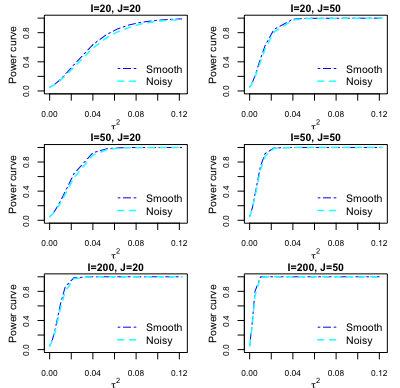
\includegraphics[width=0.9\textwidth]{powercurve.png}
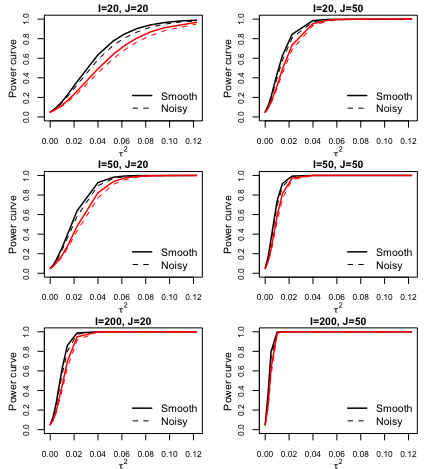
\includegraphics[width=0.9\textwidth]{bonf_homo_powercurve.png}
\caption{Power of test ($\tau_k^2\equiv\tau^2$)at the $5\%$ significance level under 12 model conditions. (1) In each panel, solid line represents that true functional data are used; dashed line represents the functional data with measurement error are used. (2) Black line denotes the power curve given by our proposed testing method assuming homogeneity of random scores; red line denotes the power curve generated by Bonferroni's correction testing method.}
\label{functional power curve}
\end{figure}
In Figure $\ref{functional power curve}$ power curves using both true and noisy $\hat{M}_{I\times J}$ across full combinations of subject number $I$ and visits $J$ are illustrated by our testing method and Bonferroni testing. Power curve is generated at each given value of common variance $\tau^2$. One can find that as subject number and visit increase, power of test will be correspondingly increased, and is able to converge to 1 eventually under each model condiction. Test of using true $\hat{M}_{I\times J}$ is always more powerful than the case when measurement error are considered, i.e. noise added $\hat{M}_{I\times J}$. If we fix the number of subjects and visits, one can easily find that our proposed method gives more powerful testing results than bonferroni's correction, as the power given by our method using noisy $\hat{M}_{I\times J}$ is always greater than Bonferroni testing using true functional data $\hat{M}_{I\times J}$ when $\tau^2$ is not too large. If we fix only one of subject number and visit number, that is, if we look at Figure $\ref{functional power curve}$ either horizontally or vertically, power curves always converge to 1 faster when the sample size is getting more. Along with this, increasing the number of visits benefits more than increasing the number of subjects in terms of stronger power. In the case of 20 subjects with 50 visits per subject, power magnitude of our test achieves at 1 when $\tau^2$ is around 0.04, whereas it comes to 0.06 when our testing gets approximately 100\% control of false positive error.

%\begin{table}[!h]
%\caption{Sizes of test at the $5\%$ level comparison (8 eigen components).  }
%\centering
%\begin{tabular}{>{\centering}p{3cm} >{\centering}p{2cm} >{\centering}p{2cm}>{\centering}p{2cm}>{\centering}p{2cm}}
%\toprule
%\multirow{2}{*}{Model condition} & \multicolumn{2}{c}{bonferroni} &  \multicolumn{2}{c}{Equal variance} \\ \cline{2-5} &$r=0$ & $r=3$ &$r=0$ & $r=3$ \tabularnewline
%\midrule
%$\text{I}=20, \text{J}=20$ & 0.051 & 0.051 & 0.051 & 0.052\tabularnewline 
%\bottomrule
%\end{tabular}
%\label{tab:sim_results for size test comparison with bonferroni(8 eigens)}
%\end{table}

%\subsection{Power Testing To Be Added}
%In the preceding simulation settings, we have shown that our testing procedure by assuming $\tau_k^2=\tau^2$ for all $k$ has good power property when the data is generated following  $\tau_k^2=\tau^2$. In this section, we use heteroscedastic variances $\tau_k^2$ over $k \in \{1,\dots, K\}$ to construct the datasets. Specifically, let $\tau_k^2=\frac{1}{2^{k-1}}\tau^2, k=1,\dots, 3$, and different nonzero $\tau_k^2$s  under the alternative hypothesis are used to generate power curves. 

\begin{figure}[h!]
\centering
%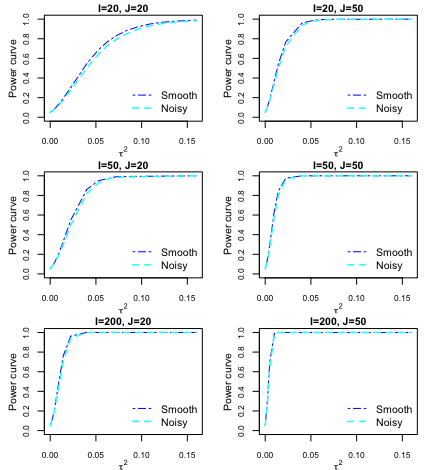
\includegraphics[width=0.9\textwidth]{heter_power_curve.png}
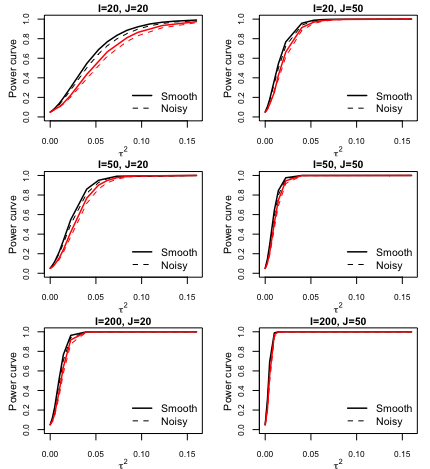
\includegraphics[width=0.9\textwidth]{bonf_heter_power.png}
\caption{Power of test ($\tau_k^2=\frac{1}{2^{k-1}}\tau^2$) at the $5\%$ significance level under 12 model conditions.(1) In each panel, solid line represents that true functional data are used; dashed line represents the functional data with measurement error are used. (2) Black line denotes the power curve given by our proposed testing method assuming homogeneity of random scores; red line denotes the power curve generated by Bonferroni's correction testing method.}
\label{heter functional power curve}
\end{figure}

Figure $\ref{heter functional power curve}$ illustrates the behavior of power when intrinsically $\tau_k^2$ increases. It shows the similar pattens with random coefficients are generated by assuming $\tau_k^2\equiv\tau^2$ for $k \in {1,\dots,3}$ under each of the conditions. That is, power of test will be increased as subject number and visit increase, and power of test will converge to 1 when $\tau^2$ is truly large (non-zero) or sample size is large enough. Under each model condition, test of using true $\hat{M}_{I\times J}$ is more powerful than using measurement error added $\hat{M}_{I\times J}$. Our testing method still outperforms Bonferroni's correction when the ramdom coefficients are truly heteroskedastic. While under heteroskedastic variance, it requires larger variance $\tau^2$ for detecting 100\% type II error compared with homogeneous variance case. 
\newpage
\subsection{Result on estimation}
Here, in order to evaluate subject-specific derivation $\beta_i(t)$ from the population effect $\beta(t)$ under heteroskedastic variance model, and compare the estimates for population effect $\beta(t)$ from heteroskedastic variance model and no functional random effect model, we consider multiple model conditions.

We generate the response $Y_{ij}$
from model \eqref{eq:lme:approx} with $K=3$, $\delta = 0.5$,
 $\gamma = 2$,
 $\gamma_i \overset{i.i.d.}{\sim} \N(0, 1)$,
 $Z_{ij} \overset{i.i.d.}{\sim} \text{Bernoulli}(0.5)$,
  $\xi_{ijk} \overset{i.i.d.}{\sim} \N(0,\lambda_k)$,
  $\theta = 2$, $\theta_{ik} \overset{i.i.d.}{\sim} \N(0, \tau_i^2)$, $i=1,\dots, K$,
  and  $\epsilon_{ij} \overset{i.i.d.}{\sim} \N(0, 1)$.
  Here, $\lambda_k=0.5^k, k=1,\dots, K$.
 Then the noisy functional data is generated from model \eqref{eq:W}
with $X_{ij}(t) = \sum_{k=1}^K \xi_{ijk} \phi_k(t)$ 
and $e_{ijk}\overset{i.i.d.}{\sim}\N(0,\sigma_W^2)$.
Here, $\phi_1 (t)=\sqrt{2}\mathrm{sin}(2\pi t)$, $\phi_2 (t)=\sqrt{2}\mathrm{cos}(4\pi t)$,$\phi_3 (t)=\sqrt{2}\mathrm{sin}(4\pi t)$, and $\sigma_W^2$ is chosen so 
that the signal to noise ratio in the functional data $r = \sigma_W^{-2}\int_{\tau} r(t,t) \mathrm{d}t$
equals either 0 or 3. Note that $r=0$ corresponds to smooth functional data without noises and 
$r=3$ corresponds to noisy functional data. Finally homogeneous $\tau_i^2$ and heteroscedastic $\tau_i^2$ are considered for variance of interest, to be specific, we take $\tau_1^2=\cdots=\tau_K^2=\tau^2, \tau^2 \in \{0.02, 0.04, 0.08\}$, and $\tau_i^2=\frac{1}{2^{i-1}}\tau^2, i=1,\dots, K, \tau^2 \in \{0.02, 0.04, 0.08\}$ separately. 

A full combination of the number of subject $I$, the number of visits per subject, $J$, the signal to noise ratio $r$ and variance of interest $\tau_i^2 (i=1,\dots,K)$ in the functional data are taken into model conditions consideration. Hence, datasets are constructed under a total of 72 different model conditions: $\big\{(I,J, r, (\tau_i^2, i=1,\dots,K), \tau^2): I\in \{ 20,50,200\}, J\in \{20,50\}, r\in \{0,3\} , (\tau_k^2,  k=1,\dots,K) \in \{ (\tau_1^2=\cdots=\tau_K^2=\tau^2), (\tau_k^2=\frac{1}{2^{k-1}}\tau^2, k=1,\dots, K) \} , \tau^2 \in \{0.02, 0.04, 0.08\} \big\}$.
Under each model condition, 1000 datasets are simulated.

ISE= $\int(\beta(t)-\hat{\beta}(t))^2 \mbox{dt}$ is used to compare estimate performance for population functional effect $\beta(t)$ from heteroskedastic variance model and no functional random effect model. MISE = $\frac{1}{I} \sum_{i=1}^{I} \int(\beta_i(t)-\hat{\beta}_i(t))^2 \mbox{dt}$ is used for evaluating the subject-specific functional random effect $\beta_i(t)$ estimated by heteroscedastic variance model. Note that ${\beta}(t) = \sum_{k=1}^{K} {\theta}{\phi}_k(t)$, ${\beta}_i(t) = \sum_{k=1}^{K} {\theta}_{ik}{\phi}_k(t), \hat{\beta}(t) = \sum_{k=1}^{K} \hat{\theta}_k\hat{\phi}_k(t)$
and $\hat{\beta}_i(t) = \sum_{k=1}^{K} \hat{\theta}_{ik}\hat{\phi}_k(t)\mathbin{,} \mbox{MSE}=\frac{1}{I} \sum_{i=1}^{I}\frac{1}{J_i} \sum_{j=1}^{J_i}(y_{ij}-\hat{y}_{ij})^2$ is used to compare predictions from heteroskedastic variance model and no functional random effect model.

\begin{table}[!h]
\caption{Estimation for heteroskedastic model with homogeneous $\tau_i^2$}
\centering
\begin{tabular}{>{\centering}p{3cm} >{\centering}p{0.2cm} >{\centering}p{1.5cm}>{\centering}p{1.5cm}>{\centering}p{0.2cm}>{\centering}p{1.5cm}>{\centering}p{1.5cm}>{\centering}p{0.2cm}>{\centering}p{1.5cm}}
\toprule
& \multicolumn{8}{c}{$ \tau_i^2 \equiv \tau^2 = 0.02$} \\ \cline{2-9} \multirow{2}{*}{Model} & \multicolumn{3}{c}{ISE for $\hat{\beta}(t)$} &  \multicolumn{3}{c}{MSE for $\hat{Y}_{ij}$} &  \multicolumn{2}{c}{MISE for $\hat{\beta}_i(t)$ } \\ \cmidrule(lr){2-4} \cmidrule(lr){5-7} \cmidrule(lr){8-9} \ \ \ & r & Without $\beta_i(t)$ & With $\beta_i(t)$ & r & Without $\beta_i(t)$ & With $\beta_i(t)$ & r & With $\beta_i(t)$  \tabularnewline
\midrule
$\text{I}=20, \text{J}=20$ & 0 & 0.0295 & 0.0295 & 0 &0.9304 & 0.8655 & 0 & 0.0662 \tabularnewline 
$\text{I}=20, \text{J}=20$ & 3 & 0.0351 & 0.0351 & 3 &1.0096 & 0.9430 & 3 & 0.0682 \tabularnewline 
$\text{I}=20, \text{J}=50$ & 0 & 0.0165 & 0.0164 & 0 &0.9928 & 0.9412 & 0 & 0.0479 \tabularnewline 
$\text{I}=20, \text{J}=50$ & 3 & 0.0187 & 0.0187 & 3 &1.0750 & 1.0228 & 3 & 0.0493 \tabularnewline 
$\text{I}=50, \text{J}=20$ & 0 & 0.0147 & 0.0147 & 0 &0.9401 & 0.8813 & 0 & 0.0581 \tabularnewline 
$\text{I}=50, \text{J}=20$ & 3 & 0.0170 & 0.0170 & 3 &1.0180 & 0.9578 & 3 & 0.0596 \tabularnewline 
$\text{I}=50, \text{J}=50$ & 0 & 0.0099 & 0.0098 & 0 &0.9929 & 0.9410 & 0 & 0.0440 \tabularnewline 
$\text{I}=50, \text{J}=50$ & 3 & 0.0108 & 0.0108 & 3 &1.0755 & 1.0237 & 3 & 0.0453 \tabularnewline 
$\text{I}=200, \text{J}=20$ & 0 & 0.0079 & 0.0080 & 0 &0.9395 & 0.8829 & 0 & 0.0527 \tabularnewline 
$\text{I}=200, \text{J}=20$ & 3 & 0.0086 & 0.0086 & 3 &1.0190 & 0.9626 & 3 & 0.0536 \tabularnewline 
$\text{I}=200, \text{J}=50$ & 0 & 0.0067 & 0.0067 & 0 &0.9945 & 0.9419 & 0 & 0.0414 \tabularnewline 
$\text{I}=200, \text{J}=50$ & 3 & 0.0070 & 0.0070 & 3 &1.0775 & 1.0249 & 3 & 0.0426 \tabularnewline 
\bottomrule
 & \multicolumn{8}{c}{$\tau_i^2 \equiv \tau^2 = 0.04$} \\ \cline{2-9} \multirow{2}{*}{Model} & \multicolumn{3}{c}{ISE for $\hat{\beta}(t)$} &  \multicolumn{3}{c}{MSE for $\hat{Y}_{ij}$} &  \multicolumn{2}{c}{MISE for $\hat{\beta}_i(t)$ } \\ \cmidrule(lr){2-4} \cmidrule(lr){5-7} \cmidrule(lr){8-9} \ \ \ & r & Without $\beta_i(t)$ & With $\beta_i(t)$ & r & Without $\beta_i(t)$ & With $\beta_i(t)$ & r & With $\beta_i(t)$  \tabularnewline
\midrule
$\text{I}=20, \text{J}=20$ & 0 & 0.0334 & 0.0331 & 0 &0.9608 & 0.8585 & 0 & 0.1067 \tabularnewline 
$\text{I}=20, \text{J}=20$ & 3 & 0.0389 & 0.0386 & 3 &1.0401 & 0.9370 & 3 & 0.1102 \tabularnewline 
$\text{I}=20, \text{J}=50$ & 0 & 0.0200 & 0.0196 & 0 &1.0253 & 0.9342 & 0 & 0.0723 \tabularnewline 
$\text{I}=20, \text{J}=50$ & 3 & 0.0221 & 0.0219 & 3 &1.1075 & 1.0162 & 3 & 0.0755 \tabularnewline 
$\text{I}=50, \text{J}=20$ & 0 & 0.0160 & 0.0159 & 0 &0.9712 & 0.8703 & 0 & 0.0975 \tabularnewline 
$\text{I}=50, \text{J}=20$ & 3 & 0.0183 & 0.0182 & 3 &1.0492 & 0.9473 & 3 & 0.1004 \tabularnewline 
$\text{I}=50, \text{J}=50$ & 0 & 0.0112 & 0.0110 & 0 &1.0260 & 0.9326 & 0 & 0.0668 \tabularnewline 
$\text{I}=50, \text{J}=50$ & 3 & 0.0121 & 0.0120 & 3 &1.1085 & 1.0152 & 3 & 0.0696 \tabularnewline 
$\text{I}=200, \text{J}=20$ & 0 & 0.0083 & 0.0083 & 0 &0.9715 & 0.8683 & 0 & 0.0905 \tabularnewline 
$\text{I}=200, \text{J}=20$ & 3 & 0.0090 & 0.0090 & 3 &1.0510 & 0.9481 & 3 & 0.0928 \tabularnewline 
$\text{I}=200, \text{J}=50$ & 0 & 0.0071 & 0.0070 & 0 &1.0280 & 0.9328 & 0 &  0.0634 \tabularnewline 
$\text{I}=200, \text{J}=50$ & 3 & 0.0074 & 0.0074 & 3 &1.1111 & 1.0156 & 3 & 0.0663 \tabularnewline 
\bottomrule
\end{tabular}
\label{tab:pred_homo_0.02_0.04}
\end{table}

\begin{table}[!h]
%\caption{Estimation results for heteroscedastic model}
\centering
%\begin{tabular}{c c c}
\begin{tabular}{>{\centering}p{3cm} >{\centering}p{0.5cm} >{\centering}p{1.5cm}>{\centering}p{1.5cm}>{\centering}p{0.5cm}>{\centering}p{1.5cm}>{\centering}p{1.5cm}>{\centering}p{0.5cm}>{\centering}p{1.5cm}}
\toprule
& \multicolumn{8}{c}{$\tau_i^2 \equiv \tau^2 = 0.08$} \\ \cline{2-9} \multirow{2}{*}{Model} & \multicolumn{3}{c}{ISE for $\hat{\beta}(t)$} &  \multicolumn{3}{c}{MSE for $\hat{Y}_{ij}$} &  \multicolumn{2}{c}{MISE for $\hat{\beta}_i(t)$ } \\ \cmidrule(lr){2-4} \cmidrule(lr){5-7} \cmidrule(lr){8-9} \ \ \ & r & Without $\beta_i(t)$ & With $\beta_i(t)$ & r & Without $\beta_i(t)$ & With $\beta_i(t)$ & r & With $\beta_i(t)$  \tabularnewline
\midrule
$\text{I}=20, \text{J}=20$ & 0 & 0.0410 & 0.0399 & 0 &1.0215 & 0.8454 & 0 & 0.1677 \tabularnewline 
$\text{I}=20, \text{J}=20$ & 3 & 0.0465 & 0.0454 & 3 &1.101 & 0.9242 & 3 & 0.1738 \tabularnewline 
$\text{I}=20, \text{J}=50$ & 0 & 0.0266 & 0.0258 & 0 &1.0899 & 0.9258 & 0 & 0.1020 \tabularnewline 
$\text{I}=20, \text{J}=50$ & 3 & 0.0289 & 0.0281 & 3 &1.1723 & 1.0079 & 3 & 0.1075 \tabularnewline 
$\text{I}=50, \text{J}=20$ & 0 & 0.0187 & 0.0183 & 0 &1.0335 & 0.8524 & 0 & 0.1546 \tabularnewline 
$\text{I}=50, \text{J}=20$ & 3 & 0.0209 & 0.0205 & 3 &1.1116 & 0.9298 & 3 & 0.1608 \tabularnewline 
$\text{I}=50, \text{J}=50$ & 0 & 0.0137 & 0.0133 & 0 &1.0919 & 0.9234 & 0 & 0.0933 \tabularnewline 
$\text{I}=50, \text{J}=50$ & 3 & 0.0147 & 0.0143 & 3 &1.1745 & 1.0060 & 3 & 0.0986 \tabularnewline 
$\text{I}=200, \text{J}=20$ & 0 & 0.0091& 0.0090 & 0 &1.0353 & 0.8482 & 0 & 0.1454 \tabularnewline 
$\text{I}=200, \text{J}=20$ & 3 & 0.0098 & 0.0096 & 3 &1.1150 & 0.9277 & 3 & 0.1507 \tabularnewline 
$\text{I}=200, \text{J}=50$ & 0 & 0.0078 & 0.0077 & 0 &1.0952 & 0.9235 & 0 &  0.0889 \tabularnewline 
$\text{I}=200, \text{J}=50$ & 3 & 0.0081 & 0.0080 & 3 &1.1782 & 1.0063 & 3 & 0.0943 \tabularnewline 
\bottomrule
\end{tabular}
\label{tab:pred_homo_0.08}
\end{table}


\begin{table}[!h]
\caption{Estimation for heteroskedastic model with hetero-variance}
\centering
%\begin{tabular}{c c c}
\begin{tabular}{>{\centering}p{3cm} >{\centering}p{0.2cm} >{\centering}p{1.5cm}>{\centering}p{1.5cm}>{\centering}p{0.2cm}>{\centering}p{1.5cm}>{\centering}p{1.5cm}>{\centering}p{0.2cm}>{\centering}p{1.5cm}}
%\toprule
\toprule
& \multicolumn{8}{c}{$\tau^2=0.02, \tau_i^2=\frac{1}{2^{i-1}}\tau^2$} \\ \cline{2-9} \multirow{2}{*}{Model} & \multicolumn{3}{c}{ISE for $\hat{\beta}(t)$} &  \multicolumn{3}{c}{MSE for $\hat{Y}_{ij}$} &  \multicolumn{2}{c}{MISE for $\hat{\beta}_i(t)$ } \\ \cmidrule(lr){2-4} \cmidrule(lr){5-7} \cmidrule(lr){8-9} \ \ \ & r & Without $\beta_i(t)$ & With $\beta_i(t)$ & r & Without $\beta_i(t)$ & With $\beta_i(t)$ & r & With $\beta_i(t)$  \tabularnewline
\midrule
$\text{I}=20, \text{J}=20$ & 0 & 0.0279 & 0.0279 & 0 &0.9234 & 0.8662 & 0 & 0.0443 \tabularnewline 
$\text{I}=20, \text{J}=20$ & 3 & 0.0335 & 0.0335 & 3 &1.0024 & 0.9433 & 3 & 0.0462 \tabularnewline 
$\text{I}=20, \text{J}=50$ & 0 & 0.0151 & 0.0151 & 0 &0.9844 & 0.9428 & 0 & 0.0293 \tabularnewline 
$\text{I}=20, \text{J}=50$ & 3 & 0.0173 & 0.0173 & 3 &1.0665 & 1.0241 & 3 & 0.0303 \tabularnewline 
$\text{I}=50, \text{J}=20$ & 0 & 0.0142 & 0.0142 & 0 &0.9325 & 0.8828 & 0 & 0.0360 \tabularnewline 
$\text{I}=50, \text{J}=20$ & 3 & 0.0165 & 0.0165 & 3 &1.0105 & 0.9589 & 3 & 0.0372 \tabularnewline 
$\text{I}=50, \text{J}=50$ & 0 & 0.0093 & 0.0093 & 0 &0.9843 & 0.9441 & 0 & 0.0262 \tabularnewline 
$\text{I}=50, \text{J}=50$ & 3 & 0.0103 & 0.0102 & 3 &1.0671 & 1.0266 & 3 & 0.0269 \tabularnewline 
$\text{I}=200, \text{J}=20$ & 0 & 0.0078 & 0.0078 & 0 &0.9315 & 0.8863 & 0 & 0.0309 \tabularnewline 
$\text{I}=200, \text{J}=20$ & 3 & 0.0085 & 0.0084 & 3 &1.0110 & 0.9656 & 3 & 0.0314 \tabularnewline 
$\text{I}=200, \text{J}=50$ & 0 & 0.0066 & 0.0066 & 0 &0.9859 & 0.9464 & 0 & 0.0241 \tabularnewline 
$\text{I}=200, \text{J}=50$ & 3 & 0.0069 & 0.0069 & 3 &1.0690 & 1.0292 & 3 & 0.0248 \tabularnewline
\bottomrule
 & \multicolumn{8}{c}{$\tau^2=0.04, \tau_i^2=\frac{1}{2^{i-1}}\tau^2$} \\ \cline{2-9} \multirow{2}{*}{Model} & \multicolumn{3}{c}{ISE for $\hat{\beta}(t)$} &  \multicolumn{3}{c}{MSE for $\hat{Y}_{ij}$} &  \multicolumn{2}{c}{MISE for $\hat{\beta}_i(t)$ } \\ \cmidrule(lr){2-4} \cmidrule(lr){5-7} \cmidrule(lr){8-9} \ \ \ & r & Without $\beta_i(t)$ & With $\beta_i(t)$ & r & Without $\beta_i(t)$ & With $\beta_i(t)$ & r & With $\beta_i(t)$  \tabularnewline
\midrule
$\text{I}=20, \text{J}=20$ & 0 & 0.0302 & 0.0301 & 0 &0.9465 & 0.8608 & 0 & 0.0670 \tabularnewline 
$\text{I}=20, \text{J}=20$ & 3 & 0.0359 & 0.0357 & 3 &1.0254 & 0.9383 & 3 & 0.0698 \tabularnewline 
$\text{I}=20, \text{J}=50$ & 0 & 0.0171 & 0.0169 & 0 &1.0085 & 0.9384 & 0 & 0.0442 \tabularnewline 
$\text{I}=20, \text{J}=50$ & 3 & 0.0193 & 0.0192 & 3 &1.0908 & 1.0198 & 3 & 0.0458 \tabularnewline 
$\text{I}=50, \text{J}=20$ & 0 & 0.0151 & 0.0149 & 0 &0.9559 & 0.8750 & 0 & 0.0582 \tabularnewline 
$\text{I}=50, \text{J}=20$ & 3 & 0.0174 & 0.0173 & 3 &1.0340 & 0.9513 & 3 & 0.0602 \tabularnewline 
$\text{I}=50, \text{J}=50$ & 0 & 0.0101 & 0.0100 & 0 &1.0088 & 0.9386 & 0 & 0.0403 \tabularnewline 
$\text{I}=50, \text{J}=50$ & 3 & 0.0110 & 0.0109 & 3 &1.0915 & 1.0210 & 3 & 0.0416 \tabularnewline 
$\text{I}=200, \text{J}=20$ & 0 & 0.0081 & 0.0080 & 0 &0.9555 & 0.8763 & 0 & 0.0525 \tabularnewline 
$\text{I}=200, \text{J}=20$ & 3 & 0.0087 & 0.0087 & 3 &1.0351 & 0.9555 & 3 & 0.0537 \tabularnewline 
$\text{I}=200, \text{J}=50$ & 0 & 0.0068 & 0.0068 & 0 &1.0110 & 0.9400 & 0 &  0.0377 \tabularnewline 
$\text{I}=200, \text{J}=50$ & 3 & 0.0072 & 0.0071 & 3 &1.094 & 1.0227 & 3 & 0.0392 \tabularnewline 
\bottomrule
\end{tabular}
\label{tab:pred_heter_0.02_0.04}
\end{table}
\begin{table}[!h]
%\caption{Estimation results for heteroscedastic model}
\centering
%\begin{tabular}{c c c}
\begin{tabular}{>{\centering}p{3cm} >{\centering}p{0.5cm} >{\centering}p{1.5cm}>{\centering}p{1.5cm}>{\centering}p{0.5cm}>{\centering}p{1.5cm}>{\centering}p{1.5cm}>{\centering}p{0.5cm}>{\centering}p{1.5cm}}
\toprule
& \multicolumn{8}{c}{$\tau^2=0.08, \tau_i^2=\frac{1}{2^{i-1}}\tau^2$} \\ \cline{2-9} \multirow{2}{*}{Model} & \multicolumn{3}{c}{ISE for $\hat{\beta}(t)$} &  \multicolumn{3}{c}{MSE for $\hat{Y}_{ij}$} &  \multicolumn{2}{c}{MISE for $\hat{\beta}_i(t)$ } \\ \cmidrule(lr){2-4} \cmidrule(lr){5-7} \cmidrule(lr){8-9} \ \ \ & r & Without $\beta_i(t)$ & With $\beta_i(t)$ & r & Without $\beta_i(t)$ & With $\beta_i(t)$ & r & With $\beta_i(t)$  \tabularnewline
\midrule
$\text{I}=20, \text{J}=20$ & 0 & 0.0350 & 0.0341 & 0 &0.9925 & 0.8513 & 0 & 0.1017 \tabularnewline 
$\text{I}=20, \text{J}=20$ & 3 & 0.0406 & 0.0398 & 3 &1.0715 & 0.9290 & 3 & 0.1060 \tabularnewline 
$\text{I}=20, \text{J}=50$ & 0 & 0.0212 & 0.0206 & 0 &1.0568 & 0.9326 & 0 & 0.0648 \tabularnewline 
$\text{I}=20, \text{J}=50$ & 3 & 0.0233 & 0.0229 & 3 &1.1392 & 1.0143 & 3 & 0.0675 \tabularnewline 
$\text{I}=50, \text{J}=20$ & 0 & 0.0167 & 0.0163 & 0 &1.0027 & 0.8630 & 0 & 0.0917 \tabularnewline 
$\text{I}=50, \text{J}=20$ & 3 & 0.0190 & 0.0187 & 3 &1.0810 & 0.9394 & 3 & 0.0952 \tabularnewline 
$\text{I}=50, \text{J}=50$ & 0 & 0.0116 & 0.0113 & 0 &1.0577 & 0.9319 & 0 & 0.0591 \tabularnewline 
$\text{I}=50, \text{J}=50$ & 3 & 0.0125 & 0.0122 & 3 &1.1405 & 1.0143 & 3 & 0.0616 \tabularnewline 
$\text{I}=200, \text{J}=20$ & 0 & 0.0085& 0.0084 & 0 &1.0035 & 0.8624 & 0 & 0.0849 \tabularnewline 
$\text{I}=200, \text{J}=20$ & 3 & 0.0092 & 0.0090 & 3 &1.0832 & 0.9414 & 3 & 0.0876 \tabularnewline 
$\text{I}=200, \text{J}=50$ & 0 & 0.0073 & 0.0072 & 0 &1.0612 & 0.9325 & 0 &  0.0556 \tabularnewline 
$\text{I}=200, \text{J}=50$ & 3 & 0.0076 & 0.0075 & 3 &1.1443 & 1.0152 & 3 & 0.0582 \tabularnewline 
\bottomrule
\end{tabular}
\label{tab:pred_heter_0.08}
\end{table}

Table $\ref{tab:pred_homo_0.02_0.04}$ and Table $\ref{tab:pred_heter_0.02_0.04}$ summarize the ISE for fixed effect $\hat{\beta}(t)$, MSE for response $\hat{Y}_{ij}$, and MISE for subject-level random effect $\hat{\beta_i}(t)$ across a total of 72 model conditions. In each scenario, compared with the model without functional random effects $\beta_i(t)$, the heteroskedastic model provides slightly smaller ISE for estimating the fixed effect $\beta(t)$, and better precision on estimating the response $Y_{ij}$ in terms of smaller MSE. Analysis using the true functional matrix ($r=0$) always outperforms modeling with biased functional matrix (r=3). As the sample size increases, both model have better performance regards smaller ISE for fixed effect estimation, smaller MSE for response prediction, and smaller MISE for subject-specific random effect estimation. In both cases of hetero-variance and homo-variance, for the heteroskedastic model, one can find that as the variance $\tau^2$ increases,  even though the estimation errors are inflated for the fixed effect $\beta(t)$ and subject-level random effect $\beta_i(t)$, prediction accuracy for the response $Y_{ij}$ keeps increasing, whereas model without functional random effect keeps working worse. Possible reasons could be that heteroskdastic model fit the data naturally better when the random coefficient underlying the data has relatively large variance, and model without functional random effect will underfit data. 






